\section{Introduction}\label{sec:introduction}
% \begin{flushright}
% \rightskip=0.8cm\textit{``Any sufficiently advanced technology is indistinguishable from magic.''} \\
% \vspace{0.2em}
% \rightskip=0.8cm---\emph{Arthur C. Clarke}
% \end{flushright}
% \vspace{1em}
The advent of Large Language Models (LLMs) such as ChatGPT\footnote{\href{https://chat.openai.com/}{https://chat.openai.com}} \cite{gpt-3.5-turbo} has profoundly transformed the landscape of automated code-related tasks \cite{chen2021evaluating}, including code completion \cite{wang2021code,lu2022reacc,guo2023longcoder,wu2024repoformer}, code translation \cite{lachaux2020unsupervised,szafraniec2022code,chen2018tree}, and code repair \cite{olausson2023self,fan2023automated,joshi2023repair,parasaram2024fact,xu2024aligning,zhang2024pydex}. 
A particularly intriguing application of LLMs is code generation, a task that involves producing source code from natural language descriptions. Despite varying definitions across studies \cite{ren2020codebleu,chen2023teaching,shojaee2023execution,wang2023codet5+}, \done{for the main scope of this survey, we focus on the code generation task and adopt a consistent definition of code generation as the natural-language-to-code (NL2Code) task \cite{austin2021program,athiwaratkun2022multi,zan2023large}.} 
\done{To enhance clarity, the differentiation between code generation and other code-related tasks, along with a more nuanced definition, is summarized in Table \ref{tab:code_tasks}.}
This area has garnered substantial interest from both academia and industry, as evidenced by the development of tools like GitHub Copilot\footnote{\href{https://github.com/features/copilot}{https://github.com/features/copilot}} \cite{chen2021evaluating}, CodeGeeX\footnote{\href{https://codegeex.cn/en-US}{https://codegeex.cn/en-US}} \cite{zheng2023codegeex}, and Amazon CodeWhisperer\footnote{\href{https://aws.amazon.com/codewhisperer}{https://aws.amazon.com/codewhisperer}}, which leverage groundbreaking code LLMs to facilitate software development.

Initial investigations into code generation primarily utilized heuristic rules or expert systems, such as probabilistic grammar-based frameworks \cite{joshi2003formalism,cohn2010inducing,allamanis2014mining,xiong2017precise,ji2020question} and specialized language models \cite{de2008z3,gulwani2010dimensions,jha2010oracle}. 
These early techniques were typically rigid and difficult to scale. 
However, the introduction of Transformer-based LLMs has shifted the paradigm, establishing them as the preferred method due to their superior proficiency and versatility.
One remarkable aspect of LLMs is their capability to follow instructions \cite{wei2022emergent,ouyang2022training,xu2023wizardlm,muennighoff2023octopack,chung2024scaling}, enabling even novice programmers to write code by simply articulating their requirements. This emergent ability has democratized coding, making it accessible to a broader audience \cite{zan2023large}. 
The performance of LLMs on code generation tasks has seen remarkable improvements, as illustrated by the HumanEval leaderboard\footnote{\href{https://paperswithcode.com/sota/code-generation-on-humaneval}{https://paperswithcode.com/sota/code-generation-on-humaneval}}, which showcases the evolution from PaLM 8B \cite{chowdhery2023palm} of 3.6\% to LDB \cite{zhong2024ldb} of 95.1\% on \texttt{Pass@1} metrics. 
As can be seen, the HumanEval benchmark \cite{chen2021evaluating} has been established as a de facto standard for evaluating the coding proficiency of LLMs \cite{chen2021evaluating}.
 
To offer a comprehensive chronological evolution, we present an overview of the development of LLMs for code generation, as illustrated in Figure \ref{fig:timeline}. 
The landscape of LLMs for code generation is characterized by a spectrum of models, with certain models like ChatGPT \cite{ouyang2022training}, GPT4 \cite{achiam2023gpt}, LLaMA \cite{touvron2023llama,touvron2023llama2}, and Claude 3 \cite{claude3} serving general-purpose applications, while others such as StarCoder \cite{li2023starcoder,lozhkov2024starcoder}, Code LLaMA \cite{roziere2023code}, DeepSeek-Coder \cite{guo2024deepseek}, and Code Gemma \cite{codegemma_2024} are tailored specifically for code-centric tasks.
The convergence of code generation with the latest LLM advancements is pivotal, especially when programming languages can be considered as distinct dialects of multilingual natural language \cite{athiwaratkun2022multi,zheng2023codegeex}. 
These models are not only tested against software engineering (SE) requirements but also propel the advancement of LLMs into practical production \cite{zhang2023unifying}.

\done{While recent surveys have shed light on code LLMs from the lenses of Natural Language Processing (NLP), Software Engineering (SE), or a combination of both disciplines \cite{zan2023large,zheng2023survey,zhang2023unifying,fan2023large,hou2024large,lyu2024automatic}, they have often encompassed a broad range of code-related tasks.} 
There remains a dearth of literature specifically reviewing advanced topics in code generation, such as meticulous data curation, instruction tuning, alignment with feedback, prompting techniques, the development of autonomous coding agents, retrieval augmented code generation, LLM-as-a-Judge for code generation, among others.
A notably pertinent study \cite{athiwaratkun2022multi,zan2023large} also concentrates on LLMs for text-to-code generation (NL2Code), yet it primarily examines models released from 2020 to 2022. 
Consequently, this noticeable temporal gap has resulted in an absence of up-to-date literature reviews that contemplate the latest advancements, including models like CodeQwen \cite{codeqwen}, WizardCoder \cite{luo2023wizardcoder}, CodeFusion \cite{singh2023codefusion}, and PPOCoder \cite{shojaee2023execution}, as well as the comprehensive exploration of the advanced topics previously mentioned.

% \begin{table}[t]
\caption{
State-of-the-art surveys on \revise{LLMs} for code.  
}
\label{tab:survey}
\centering
\scalebox{1.0}{
\rotatebox{0}{
    \begin{tabular}{lclccc}
    \toprule
        \textbf{\makecell[l]{Survey \\Reference}} & \textbf{\makecell[c]{Released \\Year-Month}} & \textbf{\makecell[l]{Code Tasks}} & \textbf{Duration} & \textbf{\makecell[c]{Techniques \\Taxonomy}} & \textbf{\makecell[c]{Latest \\Advances}}\\
    \midrule
         % Niu \textit{et al.} & 2022 &    &  & \XSolidBrush & \XSolidBrush \\
         % Niu \textit{et al.} & 2023 &    &  & \XSolidBrush & \XSolidBrush \\ 
         Zan \textit{et al.} \cite{zan2023large}  & 2023-05 & \begin{tabular}[c]{@{}l@{}}NL2Code\end{tabular} & 2020 - 2023 & \XSolidBrush & \XSolidBrush \\
         Hou \textit{et al.} \cite{hou2024large} & 2023-09 &    & 2017 - 2023 & \XSolidBrush & \XSolidBrush \\
         Zheng \textit{et al.} \cite{zheng2023survey} & 2023-11 &    &  & \XSolidBrush & \XSolidBrush \\
         Zhang \textit{et al.} \cite{zhang2023unifying} & 2024-04 &    &  & \XSolidBrush & \XSolidBrush \\
    \midrule
        Ours & 2024 & \makecell[l]{Code Generation \\(NL2Code)} & 2020 - 2024 & \CheckmarkBold & \CheckmarkBold\\
    \bottomrule
    \end{tabular}
}
}
\end{table}
\begin{table}[t] 
\caption{\done{
The applications of code LLMs in various code-related understanding and generation tasks. 
The I-O column indicates the type of input and output for each task, where C, NL, and K represent code, natural language, and label, respectively. 
Note that the detailed definitions of each task aligns with the descriptions in \cite{ahmad2021unified,austin2021program,niu2022deep,athiwaratkun2022multi,zan2023large}. 
The main scope of this survey focuses on code generation while it may involve code completion in Section \ref{sec:repository_level} and \ref{sec:retrieval_augmented}, aiming to illustrate the corresponding advancements.
% To enhance clarity, it might be beneficial for the paper to explicitly differentiate between these tasks and provide a more nuanced definition that acknowledges the varied applications of LLMs in code-related tasks.
}}
\label{tab:code_tasks}
\centering
\scalebox{0.77}{
    \begin{tabular}{clll} 
    \toprule
    \textbf{Type} & \textbf{I-O} & \textbf{Task} & \textbf{Definition}  \\
    \midrule
\multirow{12}*{Understanding} 
    & \multirow{8}*{C-K} & Code Classification & \makecell[l]{Classify code snippets based on functionality, purpose, or attributes \\ to aid in organization and analysis.} \\
    &  & Bug Detection & \makecell[l]{Detect and diagnose bugs or vulnerabilities in code to ensure \\ functionality and security.} \\
    &  & Clone Detection & \makecell[l]{Identifying duplicate or similar code snippets in software to enhance \\ maintainability, reduce redundancy, and check plagiarism.} \\
    &  & Exception Type Prediction & \makecell[l]{Predict different exception types in code to manage and handle \\ exceptions effectively.} \\
    \cmidrule{2-4}
    & C-C & Code-to-Code Retrieval & \makecell[l]{Retrieve relevant code snippets based on a given \\ code query for reuse or analysis.} \\ 
    \cmidrule{2-4}
    & NL-C & Code Search & \makecell[l]{Find relevant code snippets based on natural language \\queries to facilitate coding and development tasks.} \\
    % &  & Code Question Answering &  \\
\midrule
\multirow{15}*{Generation} 
    & \cellcolor{gray!15} \multirow{11}*{C-C} & \cellcolor{gray!15}Code Completion & \cellcolor{gray!15} \makecell[l]{Predict and suggest the next portion of code, given contextual \\information from the prefix (and suffix), while typing to enhance \\ development speed and accuracy.} \\
    &  & Code Translation & \makecell[l]{Translate the code from one programming language to another \\while preserving functionality and logic.} \\
    &  & Code Repair & \makecell[l]{Identify and fix bugs in code by generating the correct version to \\improve functionality and reliability.} \\
    &  & Mutant Generation & \makecell[l]{Generate modified versions of code to test and evaluate the \\effectiveness of testing strategies.} \\
    &  & Test Generation & \makecell[l]{Generate test cases to validate code functionality, performance,\\ and robustness.} \\
    % &  & Assert Generation & Generate a correct unit test assert statement. \\
    \cmidrule{2-4}
    & C-NL & Code Summarization & \makecell[l]{Generate concise textual descriptions or explanations of code to \\enhance understanding and documentation.} \\ 
    \cmidrule{2-4}
    & \cellcolor{yellow!40}NL-C & \cellcolor{yellow!40} Code Generation & \cellcolor{yellow!40} \makecell[l]{Generate source code from natural language descriptions to \\streamline development and reduce manual coding efforts.} \\
    \bottomrule
    \end{tabular}
}
\end{table}
Recognizing the need for a dedicated and up-to-date literature review, this survey endeavors to fill that void. We provide a systematic review that will serve as a foundational reference for researchers quickly exploring the latest progress in LLMs for code generation. 
A taxonomy is introduced to categorize and examine recent advancements, encompassing data curation \cite{wang2023self,luo2023wizardcoder,wei2023magicoder}, advanced topics \cite{parvez2021retrieval,lu2022reacc,le2022coderl,muennighoff2023octopack,liu2023rltf,chen2022codet,ni2023lever,chen2023teaching,huang2023agentcoder,shrivastava2023repofusion,zhang2023repocoder}, evaluation methods \cite{chen2021evaluating,hendrycks2021measuring,jimenez2023swe,zhuo2024ice}, and practical applications \cite{chen2021evaluating,zheng2023codegeex}. This category aligns with the comprehensive lifecycle of an LLM for code generation.
Furthermore, we pinpoint critical challenges and identify promising opportunities to bridge the research-practicality divide. Therefore, this survey allows NLP and SE researchers to seamlessly equip with a thorough understanding of LLM for code generation, highlighting cutting-edge directions and current hurdles and prospects.

The remainder of the survey is organized following the structure outlined in our taxonomy in Figure \ref{fig:taxonomy}. In Section \ref{sec:background}, we introduce the preliminaries of LLM with Transformer architecture and formulate the task of LLM for code generation. 
\done{Section \ref{sec:methodology}, we detail the systematic methodologies employed in conducting literature reviews.}
Then, in Section \ref{sec:taxonomy}, we propose a taxonomy, categorizing the complete process of LLMs in code generation. Section \ref{sec:overview} delves into the specifics of LLMs for code generation within this taxonomy framework. In Section \ref{sec:challenges}, we underscore the critical challenges and promising opportunities for bridging the research-practicality gap and conclude this work in Section \ref{sec:conclusion}. 

\begin{figure*}[p!]
\centering
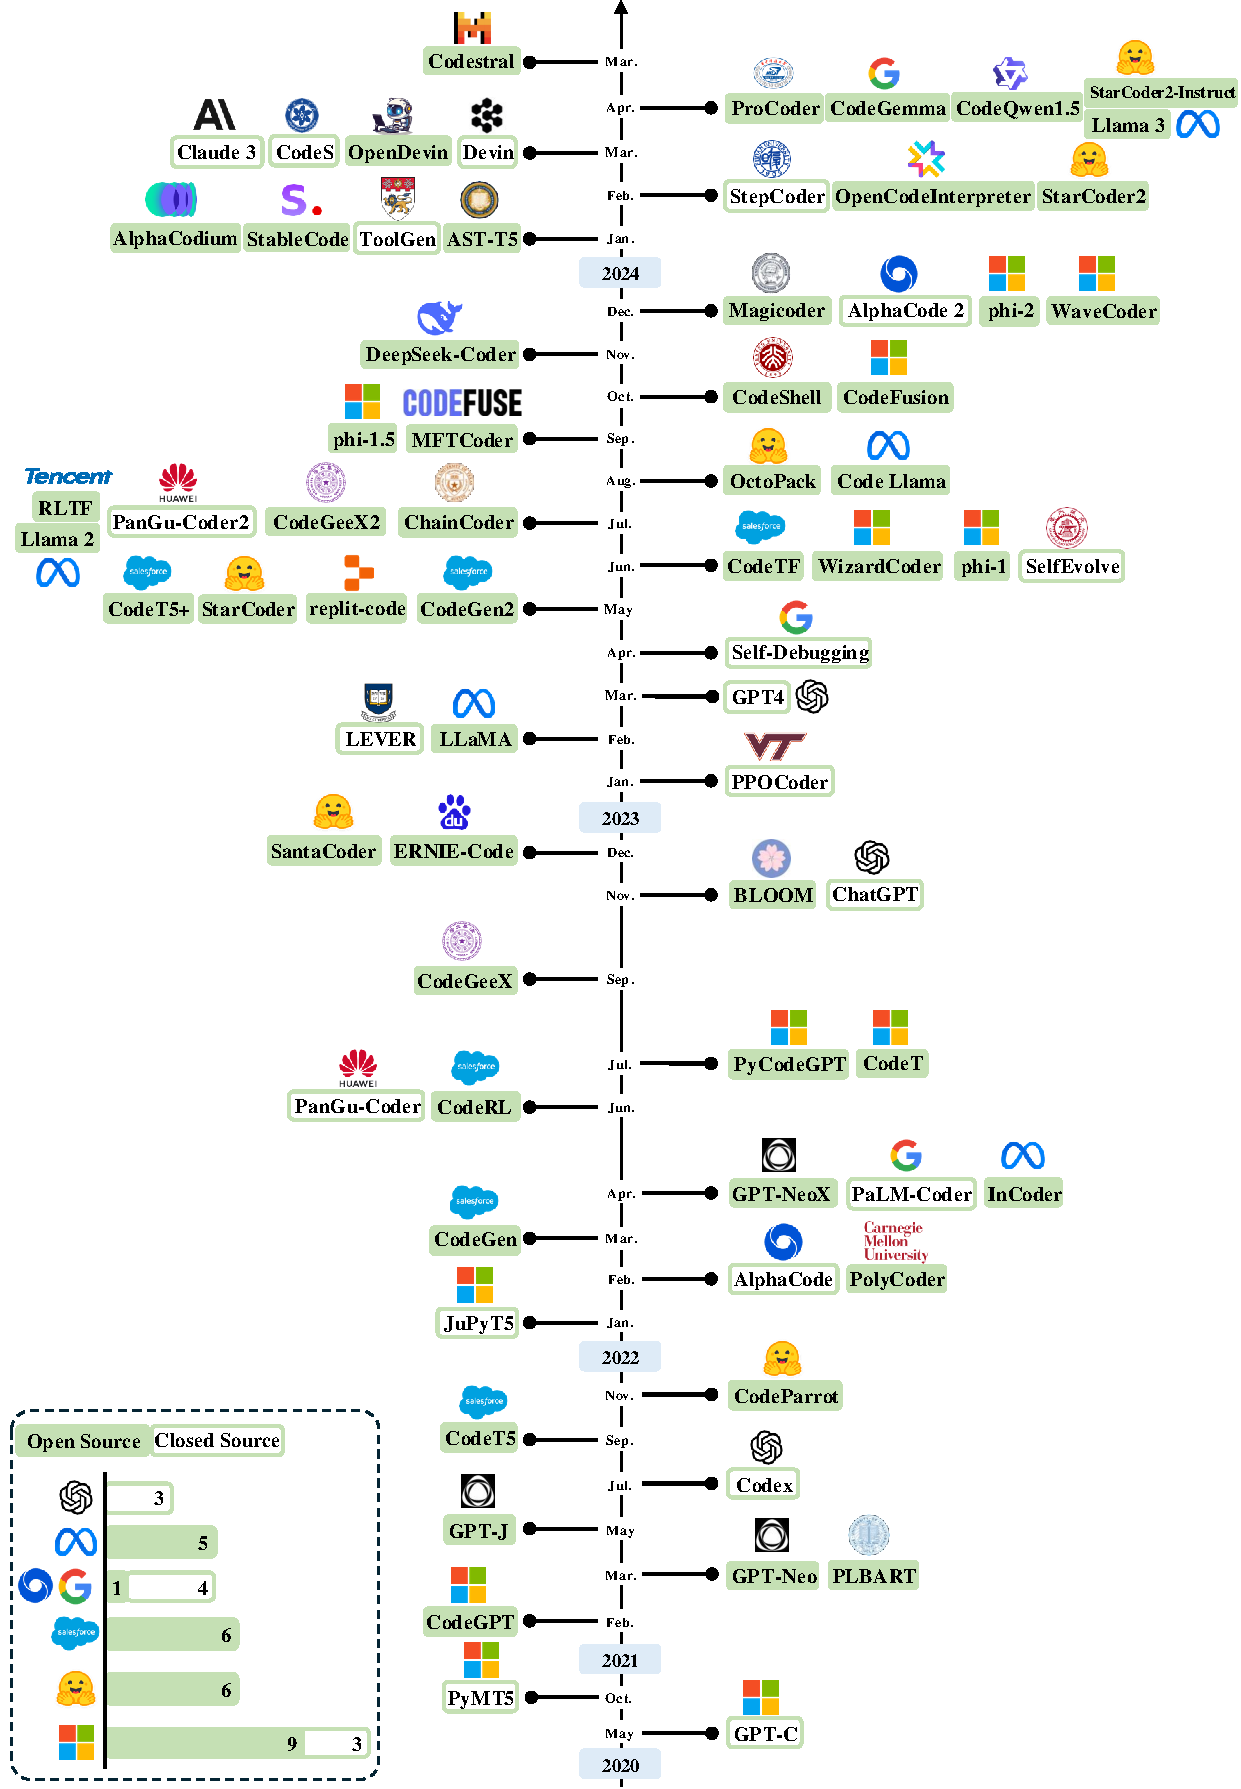
\includegraphics[width=0.97\linewidth]{images/codellm_timeline_v4.pdf}
\caption{A chronological overview of large language models (LLMs) for code generation in recent years. The timeline was established mainly according to the release date. The models with publicly available model checkpoints are highlighted in green color.}
\label{fig:timeline}
\end{figure*}